\begin{enumerate}
\item in your CLI move to the EmporioLambda Front-End\textsubscript{G} folder and use the command:\begin{center}\texttt{vercel login}\end{center}It will ask for your credentials.
\item run the command:\begin{center}\texttt{vercel link}\end{center} If you still haven't created your project on vercel it will ask you:
\begin{itemize}
\item Which scope do you want to deploy to? Choose your scope;
\item Link to existing project? Answer N;
\item What’s your project’s name? Your project name (emporio-lambda-fe);
\item In which directory is your code located? Choose the folder where your code is located.
\end{itemize}
If you already created one it will ask you:
\begin{itemize}
\item Which scope do you want to deploy to? Choose your scope;
\item Link to existing project? Answer y;
\item What’s the name of your existing project? Choose the correct project.
\end{itemize}
Other information can be found here: \url{https://vercel.com/docs/cli\#commands/overview/project-linking};
\item login into vercel website, click on the project you created and go to "Settings". Now go on "Environment Variables". Here you can set the environment variables needed for the project.\\
\begin{figure}[H]
\centering
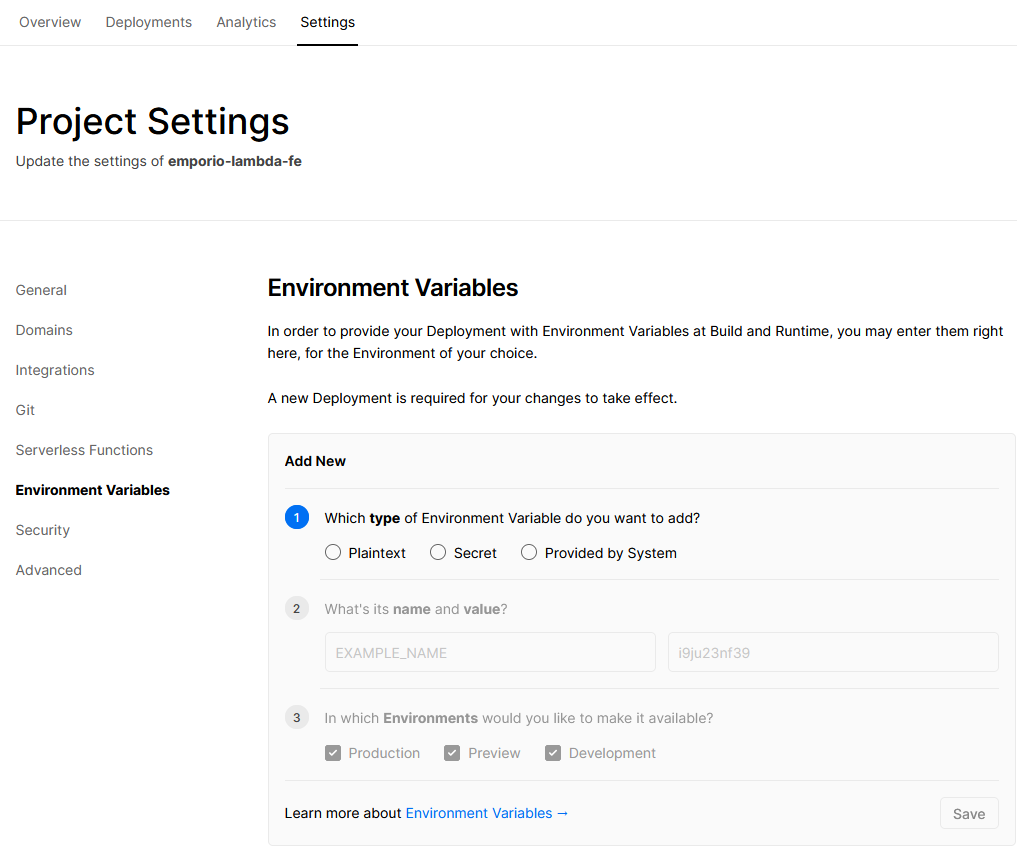
\includegraphics[scale=0.55]{res/Setup/Configurazione/img/settingsEnvVar}\\
\caption{Example of the vercel website UI}
\end{figure}
The following environment variables are needed:\\
\setcounter{table}{-1}
{
\rowcolors{2}{azzurro2}{azzurro3}
\centering
\renewcommand{\arraystretch}{1.5}
\begin{longtable}{c C{6cm} C{3cm} C{5cm}}
\rowcolor{azzurro1}
\textbf{Type} &
\textbf{Name} &
\textbf{Environment} &
\textbf{How to get/Value}\\
\endhead

Plaintext & NEXT\_PUBLIC\_STRIPE & Production, Preview, Development & Informations on how to get this variable can be found here \url{https://stripe.com/docs/keys}\\
Plaintext & NEXTAUTH\_URL & Production & Set it as your Production domain in Vercel.\\
Plaintext & COGNITO\_LOGOUT\_URL & Production & Set it as your production domain in Vercel.\\
Plaintext & COGNITO\_DOMAIN & Production & Insert here the AWS Cognito domain you use for the Production stage.\\
Plaintext & COGNITO\_CLIENT\_ID & Production & Insert here the ID of the AWS Cognito User Pool you use for the Production stage.\\
Plaintext & NEXTAUTH\_URL & Preview & Insert here the domain you use for the Preview stage.\\
Plaintext & COGNITO\_LOGOUT\_URL & Preview & Insert here the domain you use for the Preview stage.\\
Plaintext & COGNITO\_DOMAIN & Preview & Insert here the AWS Cognito domain you use for the Preview stage.\\
Plaintext & COGNITO\_CLIENT\_ID & Preview & Insert here the ID of the AWS Cognito User Pool you use for the Preview stage.\\
Plaintext & NEXTAUTH\_URL & Development & http://localhost:3000 \\
Plaintext & COGNITO\_LOGOUT\_URL & Development & http://localhost:3000 \\
Plaintext & COGNITO\_DOMAIN & Development & Insert here the AWS Cognito User Pool domain you use for the Development stage.\\
Plaintext & COGNITO\_CLIENT\_ID & Development & Insert here the ID of the AWS Cognito User Pool you use for the local stage.\\
Plaintext & NEXT\_PUBLIC\_SITE & Production & Insert here the Domain of the website for the Production stage.\\
Plaintext & NEXT\_PUBLIC\_SITE & Preview & Insert here the Domain of the website for the Preview stage.\\
Plaintext & NEXT\_PUBLIC\_SITE & Development & http://localhost:3000\\
Plaintext & NEXT\_PUBLIC\_STAGE & Production & staging\\
Plaintext & NEXT\_PUBLIC\_STAGE & Preview & test\\
Plaintext & NEXT\_PUBLIC\_STAGE & Development & local\\
Secret & NEXT\_PUBLIC\_API\_ID & Production & @next-public-api-id-staging\\
Plaintext & NEXT\_PUBLIC\_API\_ID & Preview & \\
Plaintext & NEXT\_PUBLIC\_API\_ID & Development & \\
Plaintext & NEXT\_PUBLIC\_REGION\_API & Production, Preview, Development & Insert here the location of your AWS account (example: eu-central-1). \\
Plaintext & JWT\_SIGNING\_PRIVATE\_KEY & Production, Preview, Development & run the commands:
\begin{enumerate}
\item \texttt{npm i -g node-jose-tools;}
\item \texttt{jose newkey -s 512 -t oct -a HS512;}
\item the output is the value you need.
\end{enumerate}\\
\end{longtable}
}

\item in your CLI use the command\begin{center}\texttt{vercel env pull}\end{center} This will download and setup your environment variables.
\end{enumerate}